\documentclass{beamer}
\usetheme{Singapore}
%Information to be included in the title page:
\title{Reservoir computing for the modelization of mixed effects in longitudinal data}
\author{François Plessier}
%\institute{Overleaf}
\date{4th February 2025}


\usepackage{amsmath}
\usepackage{amssymb}
\usepackage{multirow}

\usepackage{mathtools}
\usepackage{tabularx}

\usepackage[
backend=biber,
style=alphabetic,
sorting=ynt
]{biblatex}

\addbibresource{Presentation_28Nov/bibibi.bib}


\begin{document}
%\thinmuskip=6mu
\medmuskip=4mu plus 2mu minus 3mu
\thickmuskip=5mu plus 3mu minus 1mu



\frame{\titlepage}


\begin{frame}
	\tableofcontents
\end{frame}


\section{Introduction}

\subsection{Context of the study}


\begin{frame}{Context of the study}

	Context: longitudinal health data with \textbf{inter-individual heterogeneity} and \textbf{noise in the measures}.

	\bigskip


	Parametric models such as mixed effect models are commonly used.\\
	\begin{itemize}
		\item Understanding of the underlying mechanisms.
		\item However, they are sensitive to the specification.
	\end{itemize}

	\bigskip

	We consider Reservoirs Computing models:
	\begin{itemize}
		\item Neural networks adapted for time series.
		\item Able to model complex (time) relationships from "naive specifications".
		\item But… they are "black boxes" (prediction only).
	\end{itemize}


\end{frame}


\subsection{The data}

\begin{frame}{The data}


	We consider a regression problem. Synthetic datasets are used, so we can control:
	\begin{itemize}
		\item the complexity of the relationship between the variables,
		\item the inter-individual heterogeneity,
		\item the noise on the measurements.
	\end{itemize}


	\bigskip
	\bigskip
	\only<2>{
		\begin{tabular}{c}
			All the work on datasets has been done by Arthur. \\
			~                                                 \\
			\includegraphics[width=0.15\textwidth]{arthur.png}
		\end{tabular}
	}

\end{frame}




\begin{frame}{The data}

	We generate 100 training datasets (replicas), and 1 test dataset.
	\bigskip


	Each dataset has:
	\begin{itemize}
		\item repeated measures on $t \in [0,25]$ time periods
		\item for $i \in [1,500]$ individuals
	\end{itemize}

	\bigskip
	\only<2>{
	Each model is trained on each one of the 100 replicas.\\

	The resulting 100 models are then evaluated on the test dataset.\\

	We'll look at the predictions distribution and the MSE.\\

	\[ MSE = \frac{1}{N_{r}*N_{i}*N_{t}}
		\sum_{r=1}^{100}
		\sum_{i=1}^{500}
		\sum_{t=5}^{25}
		(\hat{y}_{i,t} - y_{r,i,t})^2 \]
	}


\end{frame}


\begin{frame}{The data}

	We use 7 time-dependant covariates:
	
	\begin{columns}
		\begin{column}{0.5\textwidth}	
			 \begin{align*}
		 X_{1,i}(t) = & \alpha_{0,i}^1 + \alpha_{1,i}^1 t \\ 
		 X_{2,i}(t) = & \alpha_{0,i}^2 + \alpha_{1,i}^2 log(t+1) \\ 
		 X_{3,i}(t) = & \alpha_{0,i}^3 + \alpha_{1,i}^3 t^2 \\ 
		 X_{4,i}(t) = & \alpha_{0,i}^4 + \alpha_{1,i}^4 e^{-0.002t} \\ 
		 	\end{align*}
		 \end{column}
		 \begin{column}{0.5\textwidth}	
			 \begin{align*}	
		 X_{5,i}(t) = & \frac{\alpha_{0,i}^5}{1+e^{-\alpha_{1,i}^5 t}} \\ 
		 X_{6,i}(t) = & max(0, \alpha_{0,i}^6 + \alpha_{1,i}^6 \cdot t^2) \\ 
		 X_{7,i}(t) = & \frac{\alpha_{0,i}^7}{1+e^{-\alpha_{1,i}^7 t}} \\ 
			 \end{align*}
		 \end{column}
	\end{columns}		 

	where all $\alpha_{k,i}^k$ are generated from normal distributions.

	\bigskip

	We also use a categorical covariate: $X_{8,i} = 1$ if $i$ is even else $0$\footnote{yes, it is "1~+~$i~mod~ 2$"}

\end{frame}



\begin{frame}{The data}

	We generate 1 variable of interest \textbf{without} individual effects:
	\begin{align*}
		Y^*_{fixed,i} = & \gamma_{0} +
		\gamma_{1} \cdot  X_{2,i}(t) \cdot X_{5,i}(t) + \\
		& \gamma_{2} \cdot  X_{4,i}(t) \cdot X_{7,i}(t) +
		\gamma_{3} \cdot  X_{6,i}(t) \cdot X_{8,i}
	\end{align*}

	where all $\gamma_{k}$ are generated for \textbf{all} individuals from uniform distributions.

	\bigskip

	We generate 1 variable of interest \textbf{with} individual effects:
	\begin{align*}
		Y^*_{mixed,i} = &\gamma_{0,i} +
		\gamma_{1,i} \cdot X_{2,i}(t) \cdot X_{5,i}(t) + \\
		& \gamma_{2,i} \cdot X_{4,i}(t) \cdot X_{7,i}(t) +
		\gamma_{3,i} \cdot X_{6,i}(t) \cdot X_{8,i}
	\end{align*}

	where all $\gamma_{k,i}$ are generated for \textbf{each} individuals from normal distributions.

\end{frame}






\begin{frame}{The data}

	… and we generate the corresponding noisy variables:


	\begin{align*}
		Y_{fixed,i} = & Y^*_{fixed,i} + \epsilon_{fixed,i}(t) \\
		Y_{mixed,i} = & Y^*_{mixed,i} + \epsilon_{mixed,i}(t)
	\end{align*}

	where all $\epsilon_{k,i}(t)$ are generated from normal distributions.

	\bigskip
	\only<2>{
		The trainings are done on the noisy variables.  \\
		The MSE is computed on both the noiseless and noisy variables.
	}
\end{frame}



\section{Mixed Models}

\begin{frame}{Mixed Models: modification of the prediction method}


For a fair comparison between the Mixed Models and the Reservoir Models, we consider a forecasting method, where the predictions for $t_i$ is done using only the data from $t<t_i$:

\medskip
\centering
\includegraphics[width=0.8\textwidth]{predictY.png}
\medskip


\end{frame}


\begin{frame}{Mixed Models: modification of the prediction method}


Impact of this method when considering the Mixed Effect datasets: \\

\centering
\includegraphics[width=0.8\textwidth]{fit-forecast.png}
\tiny{$$ err_{r, t} = \frac{1}{N_{i}} \sum_{i=1}^{500} (\hat{y}_{i,t} - y_{r,i,t}) $$}


\end{frame}


\begin{frame}{Mixed Models: modification of the prediction method}


Impact of this method when considering the Mixed Effect datasets: \\

\centering
\includegraphics[width=0.8\textwidth]{fit-forecast-t-polynom.png}
\tiny{$$ err_{r, t} = \frac{1}{N_{i}} \sum_{i=1}^{500} (\hat{y}_{i,t} - y_{r,i,t}) $$}

\end{frame}




\begin{frame}{Analysis of the Mixed Models results.}

Here are the MSE for the mixed effects dataset:
\medskip

\centering
\includegraphics[width=0.8\textwidth]{mixed-model-fixed.png}
\

\medskip

\begin{itemize}
	\item Impact of the specifications\\
	\item The Mixed Models use the random effects compensates the incorrect specification
\end{itemize}

\end{frame}





\begin{frame}{Analysis of the Mixed Models results.}

Here are the MSE for the fixed effects dataset:
\medskip

\centering
\includegraphics[width=0.8\textwidth]{mixed-model-mixed.png}
\

\medskip

\begin{itemize}
	\item Impact of the specifications\\
	\item The Mixed Models are efficient for correcting the noise in the observations.
\end{itemize}

\end{frame}




\section{Reservoir Computing}

\begin{frame}{Reservoir Computing}
	\begin{columns}
		\begin{column}{0.4\textwidth}
			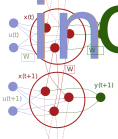
\includegraphics[width=\textwidth]{reservoir.png}
		\end{column}
		\begin{column}{0.6\textwidth}
		\begin{tabularx}{\textwidth}{lX}
			$x(t)$: & state of the Reservoir\\
			$W_{in}$: & fixed input weights\\
			$W$: & fixed recurrent weights with random initialization \newline (\textit{Echo State Property})\\
			$W_{out}$: & trainable output weights (Ridge regression)\\
		\end{tabularx}				
		\end{column}
\end{columns} 
	
	\begin{align*}
		y(t) = & ~ W_{out} ~  x(t) \\
		x(0) =  ~ 0 ~~; & ~~ x(t+1) = ~ (1-\alpha ) ~ x(t) ~ + \: \alpha \, f(u(t+1),x(t)) \\
		f(u(t+1),x(t)) = & \tanh (W_{in} \, u(t+1) \: + \: W \, x(t) ) \\
	\end{align*}




\end{frame}


\begin{frame}{Training using Reservoir Computing}


\begin{itemize}
	\item "Warm-up" steps ($N=5$) are used so the reservoir "forgets" the initialization step. \\
	\item Use of a Reservoirs ensemble from multiple ($N=5$) random seeds: $y_{pred} = 1/N_{seeds} \sum_{seeds}{y_{pred,seed}}$ \\
	\item Hyper-parameters optimization. 
\end{itemize}


\end{frame}


\begin{frame}{Hyper-parameters (HPs) optimization}

%~\cite{akiba2019optuna}
We use Optuna to optimize the main hyper-parameters of the reservoir models (Bayesian optimization):
\begin{itemize}
    \item the \textit{number of neurons} of the reservoir
    \item the \textit{leaking rate} ($\alpha$) controlling the information retention in reservoir neurons over time
    \item the \textit{spectral radius} of the reservoir, impacting its stability and memory capacity
    \item the \textit{input scaling}, which is the gain applied to the input to the reservoir
    \item the coefficient of the \textit{Ridge penalization} of the read-out layer.
\end{itemize}

\end{frame}



\begin{frame}{Hyper-parameters optimization: Pareto front}

To pickup the best set of HPs, we plot the Pareto front between the MSE on the validation set, and the number of neurons.

\begin{figure}
    \centering
    \includegraphics[height=0.7\textheight]{pareto-reservoirs-export.png}
%    \caption{Example of Pareto front for the HP optimization}
\end{figure}

\end{frame}



\begin{frame}{Hyper-parameters optimization}

We use 2 optimization steps:
\begin{enumerate}
\item one optimization using replica~\#1 as the train set and replica~\#2 as the validation set. \\ 
\item one optimization using replica~\#2 as the train set and replica~\#1 as the validation set. 
\end{enumerate}

\medskip

The final HPs are calculated as the mean of each optimization's HPs. \\

\end{frame}



\begin{frame}{Reservoir Models results}

Here are the MSE for the fixed effects dataset.
\medskip

\centering
\includegraphics[width=0.8\textwidth]{reservoir-fixed.png}
\

\medskip

\begin{itemize}
	\item More robust to the "specifications" (input).\\
	\item Also efficient at correcting the noise.
\end{itemize}


\end{frame}



\begin{frame}{Reservoir Models results}

Here are the MSE for the mixed effects dataset.
\medskip

\centering
\includegraphics[width=0.8\textwidth]{reservoir-mixed.png}
\

\medskip

\begin{itemize}
	\item It seems that we might need to use $y(t-1)$ in the input.\\
	\item Very close to the Mixed Models, on a dataset tailored for them.
\end{itemize}


\end{frame}



\begin{frame}{Reservoir Models results}



\centering
\includegraphics[width=0.8\textwidth]{reservoir-mixed-predictions.png}

\begin{itemize}
\item Higher variance for the Reservoir (Ensemble) Model.
\item Need to study a bigger Ensemble Model.
\end{itemize}

%\tiny{$$ err_{r, t} = \frac{1}{N_{i}} \sum_{i=1}^{500} (\hat{y}_{i,t} - y_{s,i,t}) $$}
\end{frame}



\section{MixedML approach}


\begin{frame}{MixedML approach}


This approach combines a Machine Learning (ML) model and a Mixed Effect model.\\
\medskip
The training is done so that:
\begin{itemize}
\item the ML model is trained to predict the fixed effects.
\item the Mixed Effect model is trained to predict the random/individual effects.
\end{itemize}

\begin{flushright}
\includegraphics[width=0.5\textwidth]{random-effects-alone.png}
\end{flushright}

\end{frame}


\begin{frame}{MixedML approach}


The training is iterative.


This approach combines a Machine Learning (ML) model and a Mixed Effect model.\\
\medskip
The training is done so that:
\begin{itemize}
\item the ML model is trained to predict the fixed effects.
\item the Mixed Effect model is trained to predict the random/individual effects.
\end{itemize}

\begin{flushright}
\includegraphics[width=0.5\textwidth]{random-effects-alone.png}
\end{flushright}

\end{frame}



\begin{frame}{MixedML approach: a lovely illustration}

\includegraphics[width=1.\textwidth]{loop_MixedML.png}

\end{frame}




\begin{frame}{MixedML approach: results}

Here are the MSE for the mixed effects dataset.
\medskip

\centering
\includegraphics[width=0.8\textwidth]{mixedML_metrics.png}

\medskip

I haven't said my last word…

\end{frame}


\begin{frame}{MixedML approach: results}
\centering
\includegraphics[width=0.8\textwidth]{mixedML-predictions.png}

\begin{itemize}
\item The variance is better than the Reservoir (Ensemble) Model.
\end{itemize}

%\tiny{$$ err_{r, t} = \frac{1}{N_{i}} \sum_{i=1}^{500} (\hat{y}_{i,t} - y_{s,i,t}) $$}
\end{frame}


\begin{frame}

\centering 
\huge{Thank you!}

\end{frame}




\end{document}